%\documentclass[English, 11pt, twoside, authoryear]{article}
%%\setlength{\columnsep}{20pt} % column separation width
%%\usepackage{txfonts} %font package that is more up to dater than times
%\usepackage{natbib}
%%\usepackage{graphicx}
%%\usepackage{wrapfig}
%\usepackage{subfigure} %% make it possible to include more than one captioned figure/table in a single float
%%\usepackage{color}
%%\usepackage{multicol}
%\usepackage{multirow}
%\usepackage{colortbl}
%%\usepackage{booktabs}
%%\usepackage{topcapt} % top caption for tables
%%\usepackage{a4wide} % makes the text on a page wider
%%\usepackage{booktabs} % for much better looking tables
%%\usepackage{paralist} % very flexible & customisable lists (eg. enumerate/itemize, etc.)
%%\usepackage{verbatim} % adds environment for commenting out blocks of text & for better verbatim
%%
%\usepackage{pdflscape}
%
%\usepackage{ctable}
%
%\newcommand{\marginal}[1]{
%	\leavevmode\marginpar{\tiny\raggedright#1\par}}
%
%%% LaTeX Preamble - Common packages
%
%%\usepackage[utf8]{inputenc} % Any characters can be typed directly from the keyboard, eg éçñ
%%\usepackage{textcomp} % provide lots of new symbols
%%\usepackage{graphicx}  % Add graphics capabilities
%%\usepackage{epstopdf} % to include .eps graphics files with pdfLaTeX
%%\usepackage{flafter}  % Don't place floats before their definition
%%\usepackage{topcapt}   % Define \topcation for placing captions above tables (not in gwTeX)
%%\usepackage{natbib} % use author/date bibliographic citations
%%
%\usepackage{amsmath} % Better maths support
%\usepackage{ulem} % more underlining and other font effects
%%usepackage{amssymb}  %  & more symbols
%%\usepackage{bm}  % Define \bm{} to use bold math fonts
%
%\usepackage[pdftex,bookmarks,colorlinks,breaklinks]{hyperref}  % PDF hyperlinks, with coloured links
%%\definecolor{dullmagenta}{rgb}{0.4,0,0.4}   % #660066
%%\definecolor{darkblue}{rgb}{0,0,0.4}
%\hypersetup{linkcolor=red,citecolor=blue,filecolor=dullmagenta,urlcolor=darkblue} % coloured links
%%\hypersetup{linkcolor=black,citecolor=black,filecolor=black,urlcolor=black} % black links, for printed output
%
%%\usepackage{memhfixc}  % remove conflict between the memoir class & hyperref
%%% \usepackage[activate]{pdfcprot}  % Turn on margin kerning (not in gwTeX)
%%\usepackage{pdfsync}  % enable tex source and pdf output syncronicity
%
%
%
%%%%% PAGE DIMENSIONS
%\usepackage[marginparwidth=3cm, top=2cm, bottom=2cm, a4paper]{geometry} % for example, change the margins to 2 inches all round
%%%\geometry{landscape} % set up the page for landscape
%%% read geometry.pdf for detailed page layout information
%\usepackage{lscape} % offers landscape environment, \begin{landscape}
%%
%
%%%%% HEADERS & FOOTERS
%\usepackage{fancyhdr} % This should be set AFTER setting up the page geometry
%\pagestyle{fancy} % options: empty , plain , fancy
%%%\renewcommand{\headrulewidth}{0pt} % customise the layout...
%\lhead{Claudius Kerth} % alined left in header
%\chead{\textbf{double digest sRAD protocol}}  % alined centrically in header
%\rhead{\today}  % alined right in header
%\usepackage{lastpage} % in order to call the number of the last page in the footer
%\lfoot{}
%\cfoot{}
%\rfoot{\thepage ~of \pageref{LastPage}}
%%
%%%%% SECTION TITLE APPEARANCE
%%%\usepackage{sectsty}
%%%\allsectionsfont{\sffamily\mdseries\upshape} % (See the fntguide.pdf for font help)
%%% (This matches ConTeXt defaults)
%%
%%%%% ToC APPEARANCE
%%%\usepackage[nottoc,notlof,notlot]{tocbibind} % Put the bibliography in the Table of Contents
%%%\usepackage[titles]{tocloft} % Alter the style of the Table of Contents
%%%\renewcommand{\cftsecfont}{\rmfamily\mdseries\upshape}
%%%\renewcommand{\cftsecpagefont}{\rmfamily\mdseries\upshape} % No bold!
%
%
%% SET UP HYPERREF
%\usepackage[pdftex,bookmarks,colorlinks,breaklinks]{hyperref}  % PDF hyperlinks, with coloured links
%%\definecolor{dullmagenta}{rgb}{0.4,0,0.4}   % #660066
%%\definecolor{darkblue}{rgb}{0,0,0.4}
%\hypersetup{colorlinks, 
%citecolor=black,% 
%filecolor=black,% 
%linkcolor=black,% 
%urlcolor=blue,% 
%pdftex}
%
%
%%
%\begin{document}
%%%%%% TITLE
%%
%\title{Double-Digest sRAD protocol}
%
%%
%%
%\author{Claudius Kerth\\University of Sheffield\\Evolutionary biology group - Prof. Roger K Butlin\\email: \texttt{c.kerth@sheffield.ac.uk}}
%%%double-shlash for line breaks
%%% \texttt sets the letters in monospace font, might be interesting for typesetting DNA sequences
%\date{\today} % tilde for no date, \today for current date
%%
%%
%%\thispagestyle{plain}
%%
%%
%%%%% BEGIN DOCUMENT
%%
%%
%\maketitle
%%
%%%Because the maketitle command has just been used, it automatically
%%%issues \thispagestyle{plain} which overrides the fancy headings for
%%%this page.  Must now tell Latex to override this!
%%
%%
%%%\tableofcontents % uncomment to insert the table of contents
%%
%
%\begin{abstract}
%This protocol describes the procedure to prepare a double-digest RAD library from genomic DNA of 38 grasshoppers. Through digestion with two restriction enzymes and ligation of the P2 adapter to one type of the sticky ends as well as through gel size selection (issue of repeatability), this protocol achieves additional complexity reduction to the standard RAD protocol by Paul Etter (Oregon). It includes a normalisation step with double strand specific nuclease usually used for cDNA libraries (Evrogen). The normalisation is recommended when the selective PCR product contains distinct bands or is severely biased towards certain fragment lengths.
%\end{abstract}
%%
%%\clearpage % inserts pagebreak, I think
%%
%% Requires the booktabs if the memoir class is not being used
%%
%%
%%%\setlength{\columnsep}{20pt} % sets the distance between the text columns
%%%\begin{multicols*}{2} % multicol package needs to be installed for this, sets the number of text columns per page to two
%%
%%
%%%%%%%%%%%%%%%%%%%%%%%%%%%%%%%%%%%%%%%%
%%\twocolumn
%%

\graphicspath{
    {/Users/Claudius/Documents/PhD/THESIS/kks32/LaTeX/Appendix1/}
    }

\section{Double-Digest sRAD protocol}

\subsection{ingredients}

{\small
\begin{itemize}
\item silica membrane genomic DNA extraction kit (e. g. Qiagen Dneasy Blood and Tissue Kit)
\item agarose
\item fluorometer, Hoechst dye and standard solutions (e. g. Calf Thymus standard)
\item SbfI High Fidelity from NEB
\item EagI HF and AgeI HF from NEB
\item thermal cycler
\item 96-well PCR plates
\item adhesive plate sealing film from qPCR machine
\item plate centrifuge
\item barcoded P1 adapters ( at 100nM concentration)
\item P2Y adapter with complementary sticky ends to the 6bp cutter used (and optionally containing barcodes)
\item \textbf{r}ATP (100nM concentration)
\item concentrated T4 DNA ligase
\item Qiagen MinElute reaction cleanup kit (Cat. no. 28204)
\item Glycerol
\item 6x OG
\item TBE
\item QG buffer
\item SybrSafe
\item Blue-light transilluminator
\item razor blades
\item SpeedVac (or just table centrifuge)
\item Phusion PCR mastermix
\item P1 and P2 PCR primer
\item filter tips
\item BioAnalyzer
\item ethidium bromide
\end{itemize}
}

%
%
\subsection{protocol}
%
%

\subsection{isolate DNA from grasshopper hindleg}
\begin{itemize}
\item with Qiagen Dneasy Blood and Tissue Kit (spin columns)
\end{itemize}

\subsection{check the quality of the isolations}
\begin{itemize}
\item by running each isolation on a 1.0\% gel
\end{itemize}

%\begin{figure}[!htb]
%\begin{center}
%\includegraphics[scale=0.5]{DNAiso180410_cropped}
%\caption{Four spin column DNA isolation from grasshopper hindlegs next to HindIII digested lambda. The DNA is obviously already fragmented. All grasshopper DNA isolations look like that. The sRAD protocol worked anyway fine with them.}
%\label{DNAiso}
%\end{center}
%\end{figure}

\subsection
{quantify DNA samples with fluorometer twice}
\begin{itemize}
\item produce at least three replicates of calf thymus standard serial dilutions for the standard curve
\item produce at least 5 points for the standard curve spanning from $\sim$200ng/$\mu$l to $\sim$12.5ng/$\mu$l
\item remove dodgy measurements of the standard in order to increase $r^{2}$ to at least 0.99
\item get at least two concentration measurements per DNA isolation
\end{itemize}

\subsection
{digest 132 ng of DNA from each individual with SbfI HF and XhoI}
\begin{itemize}
\item make master mix of 40$\times$:
	\begin{itemize}
	\item 3.0$\mu$l 10X NEBuffer 4
	\item 3.0$\mu$l 10x BSA 
	\item 0.5$\mu$l SbfI-HF (20 U/$\mu$l) $\rightarrow$ 10 U/sample $\rightarrow$ 72U/$\mu$g DNA \footnote{This requires 20$\mu$l of the 25$\mu$l SbfI enzyme in a tube of 500 U.}
	\item 0.5$\mu$l XhoI (20 U/$\mu$l) $\rightarrow$ 10 U/sample $\rightarrow$ 72U/$\mu$g DNA
	\item 10$\mu$l ddH$_{2}$O
	\end{itemize}
\item based on the DNA measurements, adjust the amount of DNA isolation volume for the digestion, so that more or less equal amounts of each sample go into the library (see \texttt{Fluorimeter.ods})
\item fill with ddH$_{2}$O to 30$\mu$l endvolume
\item the total amount of DNA from all samples should not exceed the capacity of a MinElute spin column (5$\mu$g). Otherwise, two separate libraries have to be prepared.
\item in an Excel spreadsheet, enter the code and volume of each DNA isolation in a layout that corresponds to the 96 well plate, print it out and use it as reference when pipetting
\item beware of cross-contamination, particularly when opening the lid of the plate
\item mix by pipetting, shake the plate at the end, spin down with centrifuge
\item incubate for 3 hours at 37$^{\circ}$C in a thermal cycler with heated lid
\item heat-inactivate in thermal cycler at 65$^{\circ}$C for 20 min, then ramp down to room temperature at no more than 2$^{\circ}$C/min \footnote{adhesive films for qPCR plates only seal tight after heating via a heated lid beyond 70$^{\circ}$C}
\end{itemize}

\subsection
{calculate the molar amount of sticky ends in the restriction digest}
\begin{itemize}
\item Parameters:
	\begin{itemize}
	\item genome size: $12\times10^{9}$bp
	\item average molecular weight of a base pair: 660$\frac{g}{mol\times bp}$
	\item expected number of SbfI restriction sites per genome (GC 46.5\%): 135,633 \footnote{see \texttt{ComplexityReduction.xls} for the calculation of this number }
	\item amount of digested DNA in g per sample: $132\times 10^{-9}$g
	\end{itemize}

\item SbfI sticky ends:
% in order to be able to use the 'equation' environment you need to load the package 'amsmath'
% load package 'ulem' for \uuline command
\begin{align}
\text{molar amount of SbfI sticky ends} &= \frac{\text{amount of DNA}}{\text{MW of bp} \times \text{genome size} } \times \text{SbfI sites per genome} \times 2 \\ \nonumber 
							   &= \frac{132\times 10^{-9}g}{660 \frac{g}{mol\times bp} \times 12\times10^{9} bp} \times 135,633 \times 2\\ \nonumber
							   &= 4.52 \times 10^{-15} \text{mol}\\ \nonumber
							   &= \uuline{4.52 \text{fmol per sample}}
\end{align}

\item XhoI sticky ends:
	\begin{itemize}
	\item expected number of XhoI restriction sites per genome (GC 46.5\%): \\ 2,509,115 \footnote{see \texttt{ComplexityReduction.xls} for the calculation of this number } $\rightarrow 18.5 \times \text{SbfI sites}$ 
	\begin{align}
	\text{molar amount XhoI sticky ends} &= 18.5 \times \text{molar amount of SbfI sticky ends} \\ \nonumber
								&= 18.5 \times 4.52 \times 10^{-15} \text{mol} \\ \nonumber
								&= 83.6 \times 10^{-15} \text{mol} \\ \nonumber
								&= \uuline{83.6\text{fmol per sample}}
	\end{align}
	\end{itemize}
\item in order to provide adapters in $\sim10-20 \times$ excess toward sticky ends, use 100fmol (=0.1pmol) P1 adapter per sample and 2pmole of P2 adapter per sample
\end{itemize}

\subsection
{set up a 10$\mu$M P2Y-XhoI adapter stock solution from oligos}
\begin{itemize}
\item set up annealing buffer (AB) as shown in table \ref{AB} \marginal{{\color{red}does this buffer contain a high enough salt concentration?!}}
\marginal{{\color{blue}yes, 1X NEB2 contains 50mM NaCL}}
% call ctable package, 
\ctable[ 
	caption =  {annealing buffer set up:},
	label = AB,
	pos = htb!,
	width = 70mm,
%	captionskip = -.5ex, % bring the caption closer to the table
	center
]
{>{\raggedright}X>{\raggedleft}X}
{
\tnote{1x NEB2 contains 10mM MgCl$_{2}$}
\tnote[b]{0.372g EDTA dissolved in 10ml 1x NEB2}
}
{
\FL
NEB2 (10x)\tmark		&	100$\mu$l 	\NN
EDTA (100mM)\tmark[b]	&	110$\mu$l 	\NN
ddH$_{2}$O			& 	790$\mu$l	\ML
					&	1,000$\mu$l
\LL
}
\item \dots split the volume into 100$\mu$l aliquots and heat them to 65$^{\circ}$ for 20 minutes \footnote{in order to denature nuclease contamination}
\item spin down lyophilised oligos in manufacturers tube for 1 min at maximum speed
\item dissolve the lyophilised oligos with EB to 100$\mu$M
\item then set up 10$\mu$M adapter solution with:
\ctable[ 
	caption =  { },
%	label = ,
	pos = h,
	width = 80mm,
%	captionskip = -.5ex, % bring the caption closer to the table
	center
]
{>{\raggedright}X>{\raggedleft}X}
{ }
{
\FL
upper oligo (100$\mu$M)	&	10$\mu$l 	\NN
lower oligo (100$\mu$M)	&	10$\mu$l 	\NN
AB					& 	80$\mu$l	\ML
					&	100$\mu$l
\LL
}
\item \ldots and anneal the oligos by heating the mixture in the thermal cycler to 96$^{\circ}$C for 2 minutes and then ramping down to RT at 2$^{\circ}$/min

\end{itemize}

\subsection
{ligate adapters to each restriction digest}
\begin{itemize}
\item put the sample plate on ice
\item thaw P1 adapter plate on ice, shake to mix, spin down, reseal the plate after use
\item first add to each heat inactivated restriction digest:
	\begin{itemize}
	\item 1.0 $\mu$l of 100nM barcoded P1 adapter $\rightarrow$ 0.1 pmol \footnote{0.757pmole/$\mu$g DNA; 22 fold excess of adapter to cohesive ends. If you size select at 300bp or above, adapter dimers shouldn't be a problem.}
	\item 2.0 $\mu$l of 1$\mu$M P2-XhoI adapter $\rightarrow$ 2.0 pmol \footnote{15 pmol/$\mu$g DNA; 23.9 fold excess of adapter to cohesive ends.}
	\end{itemize}
\item vortex plate and spin down
\item then make master mix of 40$\times$:
\begin{itemize}
\item 0.8 $\mu$l 10X NEB Buffer 2 \footnote{adds 10mM NaCl to the final solution, final NaCl concentration $\sim$50mM, which is necessary to keep the P2Y adapter double stranded; however, salt concentrations of 100mM decrease ligation efficiency (from NEB FAQ)}
\item 0.4 $\mu$l \textbf{r}ATP (100mM $\rightarrow$ end concentration 1 mM) \footnote{rATP powder dissolved in EB (pH 8.5) is stable; reduce freeze-thawing cycles;  0.1 mM ATP is as efficient as 1mM but a 10mM ATP concentrations inhibit ligations!}
\item 0.2 $\mu$l concentrated T4 DNA Ligase (2,000 NEB U/$\mu$l) \footnote{400U/sample corresponding to 3030 NEB U/$\mu$g DNA}
\item 5.6 $\mu$l ddH$_{2}$O
\end{itemize}
\item add 7.0 $\mu$l of master mix to each well to a 40$\mu$l end volume and mix by pipetting up and down
\item after carefully sealing the plate with adhesive film, vortex and spin down
\item final monovalent cation concentration should be $\sim$50 mM \footnote{NEBuffer 4 contains 50mM potassium ions}
\item incubate at room temperature (RT) for 2 hours, then over night in the fridge
\item heat-inactivate at 65$^{\circ}$C for 20 min in thermal cycler, then ramp down to RT at 2$^{\circ}$C/min
\end{itemize}

\subsection
{combine samples}
\begin{itemize}
\item pool the 38 individual ligation mixes, making up $\sim$1,520$\mu$l and $\sim$5 $\mu$g DNA 
\end{itemize}

%%%%% ctable - for tables with footnotes. Very useful. 
% call ctable package, 
%\ctable[ 
%	caption = optimal Covaris settings,
%	label = Covaris,
%	pos = h,
%	width = 55mm,
%	captionskip = -2ex, % bring the caption closer to the table
%	center
%]
%{>{\raggedright}X>{\raggedleft}X}
%{}
%{
%\FL
%duty cycle		&	10\% 	\NN
%intensity		&	5 		\NN
%cycles/burst	& 	200		\NN
%duration		&	100sec
%\LL
%}

%\item optimal Covaris settings:
%\begin{tabular}{lr}
%\hline \addlinespace[.5em]
%duty cycle	&10\%\\
%intensity	&5\\
%cycles/burst	&200\\
%duration		&100sec\\
%\addlinespace[.5em] \hline 
%\end{tabular}
%\end{itemize}


\subsection
{clean up and concentrate the adapter ligated library}
\begin{itemize}
\item with one Qiagen MinElute reaction cleanup column (Cat. no. 28204), capacity each 5$\mu$g DNA\footnote{ignore what the kit manual says about the maximum amount of enzymatic reaction that can be cleaned up per column}
\item use at least as much ERC buffer as ligation mix for the reaction cleanup kit 
\item elute with 15 $\mu$l EB
\end{itemize}

\subsection
{size selection on agarose gel}\label{sizeSelection}
\begin{itemize}
\item rinse the gel tank and use fresh buffer before running the gel\footnote{if you have run a gel from a different library before, otherwise not necessary} 
\item make a 110ml 1\% TBE gel with 6.3$\mu$l SybrSafe
\item add 10$\mu$l 6x OG loading dye and $\sim$5$\mu$l 100\% Glycerol to the 15$\mu$l eluate of the last step \footnote{$\sim$5$\mu$g DNA per lane, the glycerol is necessary to make the DNA sink into the gel well, a lot of DNA could otherwise be lost at this step}
\item run the whole mix in one lane at 13 V/cm for $\sim$45 min or when the orange dye just about reaches the bottom of the gel
\item the wells should be less than half full, otherwise migration of fragments will be distorted $\rightarrow$ 5--6mm wide wells
\item load 30$\mu$l 100bp ladder (50ng/$\mu$l) in the left lane, leave 1 lane space between standard and library
\item use fresh razor blade and a blue light transilluminator to cut out a size range of $\sim$300-800 bp (fig. \ref{SizeSel}) \footnote{be as accurate as possible with the vertical cuts, you can take your time, be sure not to go below 300bp, otherwise risk of adapter dimer contamination (Maureen Liu)}
\item cut the gel block into 4 pieces and put each into a 2ml tube
\item weigh each tube and subtract the weight of an empty tube to get the gel weights in mg
\item add $3 \times$ as much buffer QG to each tube as the weight of its gel piece
\item rotate the tubes at RT for one hour to melt the gel pieces 
\item combine the dissolved gel pieces in a bigger vessel and add one gel volume (mg=ml) of isopropanol followed by mixing
\item purify that solution over one MinElute spin column with a SpeedVac \footnote{even though it says otherwise in the manual of the kit, you can gel extract with just one column as long as the gel contains no more than 1\% agarose and it is completely melted before loading}
\item elute with 30$\mu$l EB
\end{itemize}

\begin{figure}[!htb]
\begin{center}
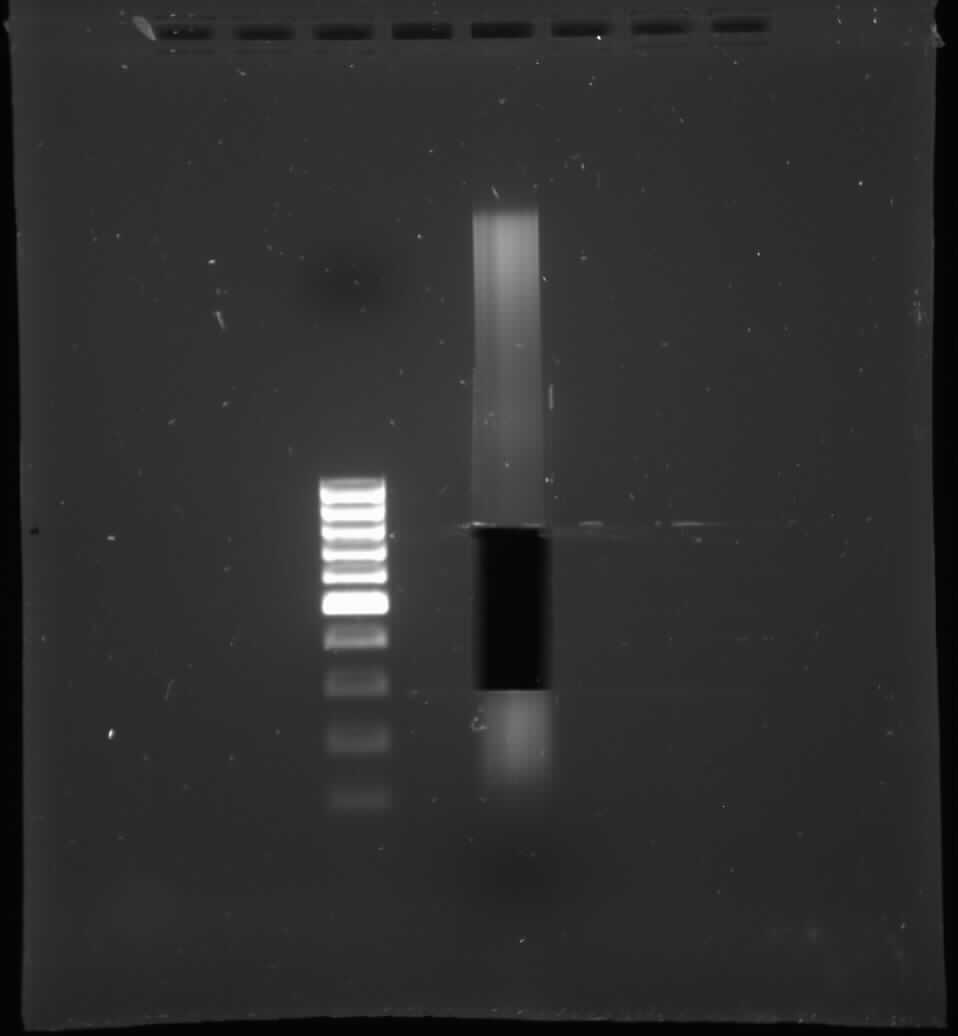
\includegraphics[scale=0.3]{GelSizeSelection_071011}
\caption{Gel picture after size selection.}
\label{SizeSel}
\end{center}
\end{figure}

%\begin{figure}[!htb]
%\begin{center}
%\subfigure[two pools sheared with the Covaris settings from Table \ref{Covaris}]{\label{shearedPools}\includegraphics[scale=0.32]{shearedPools_180610_1}}
%\hfill
%\subfigure[after size selection of the pools]{\label{shearedPools}\includegraphics[scale=0.3]{sizeSelection_after_250610}}
%\caption{Size selection of fragments after shearing.}
%\label{shearedPools}
%\end{center}
%\end{figure}

\subsection
{selective amplification}
\label{selAmp}
\begin{itemize}
\item save 6$\mu$l of the eluate of the last step for later qPCR
\item then set up a PCR with the remaining 24$\mu$l eluate:
	\begin{itemize}
	\item 6.0 $\mu$l H2O
	\item 50.0 $\mu$l 2x Phusion Mastermix \footnote{Do not use Phusion PCR kit with standard dNTP's. Phusion only works with high quality dNTP's !}
	\item 10.0 $\mu$l P1-thiol primer (10$\mu$M) $\rightarrow$ 1.0$\mu$M end concentration \footnote{I found that a much higher primer concentration than usual can greatly increase yield}
	\item 10.0 $\mu$l P2-thiol primer (10$\mu$M)
	\item 24 $\mu$l RAD library template
	\end{itemize}
\item split the PCR mix into 5x 20$\mu$l volumes and add 10$\mu$l mineral oil to each PCR tube
\item then run each tube with the PCR programme shown in table \ref{selPCR}
%%%%% ctable - for tables with footnotes. Very useful. 
% call ctable package
\ctable[ 
	caption = PCR programme,
	label = selPCR,
	pos = h,
	width = 45mm,
	center
]
{>{\centering}X>{\raggedright}X>{\raggedright}X}
{
	\tnote{30sec per kb recommended}
}
{
					\FL
98$^{\circ}$  & 30sec	 &	 \ML
98$^{\circ}$  & 10sec	 & 
\multirow{3}{*}{\Huge{$\}$}\normalsize$\times$18} \NN
65$^{\circ}$  & 30sec	 &	\NN
72$^{\circ}$  & 30sec\tmark[a] &\ML 
72$^{\circ}$ & 5min	&	\NN
4$^{\circ}$  & $\infty$	&	\LL
}
\end{itemize}

\subsection
{purifcation and concentration of the selective PCR product}
\begin{itemize}
\item {\color{red}use filter-tips or different pipettes for anything post-PCR !}
\item combine all PCR products and check 5$\mu$l of it on a 1.25\% gel next to 2$\mu$l Genruler
\item take 6$\mu$l of the PCR product for qPCR
\item purify the rest of the PCR product over a MinElute column eluting with 10$\mu$l EB
\end{itemize}

\subsection
{determination of template amount used for selective PCR by qPCR}
\begin{itemize}
\item {\color{red}use filter-tips}
\item use 4$\mu$l of the 6$\mu$l of the PCR product set aside in the previous step to determine it's DNA concentration with the fluorometer and picoGreen dye and use it as a standard in the qPCR
\item make 8x 1:10 serial dilutions of the PCR product in 10$\mu$l EB each to produce a standard curve
\item set up 20$\mu$l qPCR reactions with SybrGreen PCR master mix and 2$\mu$l template: 
	\begin{itemize}
	\item three replicates of serial dilutions including negative control
	\item three replicates of the template saved in step \ref{selAmp}
	\end{itemize}
\item from the C$_{t}$ values and the known amount of template molecules in the standard dilution, determine the amount of template molecules per locus and individual \footnote{This can be used to predict the expected proportion of false homozygote genotype calls due to PCR drift and false heterozygote genotype calls due to high coverage PCR mutations.} \\(see \texttt{sRAD/qPCR/TRIAL\_LIB\_241011\_data.xls})
\end{itemize}


\subsection
{normalisation of the library}
Unless the library looks like a homogeneous smear on the gel, it is advisable to normalise it.
\begin{itemize}
\item check activity of double strand specific nuclease (DSN) with control template from the kit
\item {\color{red}use filter-tips}
\item take 6$\mu$l of the purified PCR product and add 2$\mu$l 4x Hybridization buffer \footnote{500mM final NaCl concentration for annealing. EB contains 10mM Tris-HCl at pH 8.5, 1x hybridization buffer contains 50mM HEPES at pH 7.5. So the pH in the mixture should be close to 7.5.}
\item put 4$\mu$l of the mixture in each of two tubes, labeled ``1/8'' and ``1/16''
\item overlay the reaction mixtures with 10$\mu$l mineral oil and spin down for 2 min at max speed
\item in a thermal cycler, heat the mixture to 98$^{\circ}$ for 2 min
\item \ldots then incubate at 68$^{\circ}$ for 5 hours
\item put DSN master buffer into thermal cycler to preheat it to 68$^{\circ}$
\item make a 1/8th and 1/16 dilution of the DSN enzyme with DSN storage buffer
\item keep the thermal cycler at 68$^{\circ}$C and add 5$\mu$l preheated DSN master buffer to each tube while keeping the tube in the cycler, then flick, spin down briefly and immediately put back into the thermal cycler 
\item incubate for 10 minutes at 68$^{\circ}$C 
\item add 1$\mu$l of 1/8th or 1/16th DSN enzyme into each tube respectively \footnote{just add the enzyme, don't flick, don't spin down, just be quick, i. e. no more than 10 seconds for this step!}
\item incubate for 25 minutes at 68$^{\circ}$C 
\item add 10$\mu$l DSN stop solution, mix and spin \footnote{the reaction mixture contains 5mM MgCl$_{2}$ and the stop solution contains 5mM EDTA to neutralise it. Figure 4(B) in the TRIMMER kit manual suggests that inactivation of DSN by heating is not guaranteed to be complete.}
\end{itemize}

\subsection
{test PCR of normalisation}
\begin{itemize}
\item {\color{red}use filter-tips}
\item from each vial of the last step (i. e. ``1/8'' and ``1/16''), set up three 10$\mu$l test PCR's with 1$\mu$l template
\item run PCR for 5, 10 and 15 cycles with temperature steps as in table \ref{selPCR} and check 5$\mu$l PCR product on a 1.25\% EtBr gel next to 2$\mu$l Genruler
\item examine the PCR product: homogeneous smear in right size range?, 5 cycle PCR product visible? (see figure \ref{NormTestPCR})

\begin{figure}[!htb]
\begin{center}
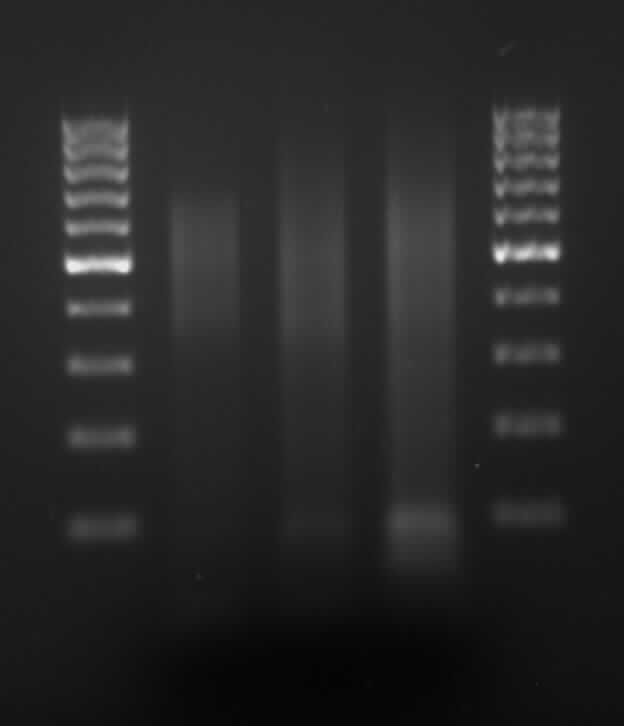
\includegraphics[scale=0.4]{Normalisation_test_lib_PCR_28072011}
\caption{Gel picture of 5, 10 and 15 cycle test PCR's (from left to right).}
\label{NormTestPCR}
\end{center}
\end{figure}

\item decide which DSN dissolution produced the better result
\end{itemize}

\subsection
{amplification of normalised library}
\begin{itemize}
\item {\color{red}use filter-tips}
\item set up a 50$\mu$l PCR as follow:
	\begin{itemize}
	\item 25$\mu$l 2x Phusion Master mix
	\item 5$\mu$l P1-thiol primer (10$\mu$M)
	\item 5$\mu$l P2-thiol primer (10$\mu$M)
	\item 10$\mu$l normalised library
	\item 5$\mu$l ddH$_{2}$O
	\end{itemize}
\item run the PCR programme in table \ref{selPCR} for 5-7 cycles, depending on the outcome of the test PCR \footnote{These additional PCR cycles do not further bias the library's representation of the pre-normalisation template since this PCR starts with a lot of template molecules as indicated by the few cycles necessary to create a visible PCR product.}
\end{itemize}

\subsection
{purification of the library}
\begin{itemize}
\item {\color{red}use filter-tips}
\item purify the 50$\mu$l PCR product over a MinElute column
\item elute with 25$\mu$l EB
\item use 4$\mu$l for DNA concentration measurement with fluorometer
\item calculate an estimate of the molar concentration of the library
\end{itemize}

%\begin{figure}[!htb]
%\begin{center}
%\includegraphics[scale=0.5]{selPCR_260610_cropped}
%\caption{PCR products of test amplifications of two libraries left of their respective templates. Adapter dimers are visible at $\sim$130bp.}
%\label{testAmp}
%\end{center}
%\end{figure}

%\subsubsection
%{perform a 100$\mu$l PCR}
%\begin{itemize}
%\item with 4$\mu$l template if very strong PCR product from test PCR, otherwise up to 30$\mu$l template
%\item 18 PCR cycles only in order to minimize PCR duplicates and bias
%\item purify the PCR product with Qiagen MinElute PCR purification column, elute with 20$\mu$l
%\item use filter-tips for anything post-PCR !
%\end{itemize}
%
%\subsubsection
%{gel purification of amplified library}
%\begin{itemize}
%\item use filter-tips for anything post-PCR !
%\item rinse the gel tank and use fresh buffer before running the gel if you have run a different library before
%\item run elution (20$\mu$l) in one lane of 1.25\% agarose gel with 10 $\mu$l 6X Orange Dye for 1h 15 min at 6.7 V/cm
%\item the wells should be less than half full, otherwise migration of fragments will be distorted \footnote{5--6mm wide wells}
%\item load 20$\mu$l 100bp ladder (20$\mu$g) in the left lane, leave 1 lane space between standard and library
%\item use fresh razor blade and UV transilluminator (long wave setting to minimize mutations) to cut out a size range of $\sim$350-750 bp \footnote{adapter dimers run at $\sim$130bp, when making the vertical cuts, be sure not to go below 350bp, otherwise risk of adapter dimer contamination (Maureen Liu)}
%\end{itemize}
%
%%\begin{figure}[!ht]%a picture has to be inserted into a figure environment in order to make it floatable; a star at figure has to be added for a two column layout
%%\begin{center}
%%\subfigure[before size selection]{\label{before}\includegraphics[scale=0.5]{selPCR_040710_gel_before_cropped}}
%%\hfill %pushes the graphics to the left and right margins
%%\subfigure[after size selection]{\label{after}\includegraphics[scale=0.5]{selPCR_040710_gel_after}}
%%\end{center}
%%\caption{Size selection of the amplified RAD library. Adapter dimer bands are clearly visible. About $\sim$0.03\% of the reads from this library came from adapter dimers or sequences with very small genomic inserts.}
%%\label{sizeSelection2}%the label command has to occur after the caption but inside the figure environment to refer (with \ref) to the figure and not the section of the document
%%\end{figure}
%
%
%\subsubsection
%{gel extraction}
%\begin{itemize}
%\item filter-tips !
%\item with MinElute Gel Extraction Kit
%\item melt agarose slice at room temperature with frequent mixing
%\item elute in 20 $\mu$l EB
%\end{itemize}
%
%
%
%\subsubsection
%{quantify molar concentration of RAD tags}
%\begin{itemize}
%\item determine DNA concentration of the library with fluorimeter twice and each with at least 3 replicates of the calf thymus standard serial dilution
%\item determine size distribution and peak size of RAD tags with Agilent Bioanalyzer 2100 DNA chip or from agarose gel picture
%\item multiply peak size by 650 [g/mol] \footnote{the molecular weight of a base pair} to get the molecular weight of the library
%\item divide the DNA concentration of the library [g/$\mu$l] by it's molecular weight to get the molar concentration [nmole/L] of RAD tags in the library
%\end{itemize}
%
\subsection
{validate library \protect \footnote{optional because of the cost and effort involved with cloning, but recommended before spending a lot of money on Solexa sequencing}}
\begin{itemize}
\item A-tail PCR product
\item T/A clone 1.0 $\mu$l of library into pGEM vector
\item Sanger sequence a few dozen clones
\item check for whether the sequences contain a P1 adapter sequence on one end and a P2 adapter sequence on the other
%\item also check for the frequency of PCR duplicates among the clones\footnote{when P2Y adapter is at the same position in two clone sequences} and blast the sequences
\end{itemize}

\pagebreak

\begin{landscape}

\ctable[ 
	caption =  {comparison among different ddRADseq protocols},
	label = compProt,
%	pos = htb!,
%	sideways,
	width = 240mm,
	captionskip = 1ex, % bring the caption closer to the table
	doinside=\footnotesize,
	center,
]
{l>{\raggedright}X>{\raggedright}X>{\raggedright}X>{\raggedright}X>{\raggedright}X>{\raggedright}X>{\raggedright}X}
{
}
{
\FL
\textbf{protocol}   &   \textbf{adapters}   &   \textbf{DNA isolation}   &   \textbf{digestion}   &   \textbf{ligation}   &   \textbf{gel size selection}   &   \textbf{PCR}   &   \textbf{purification}
\ML
\cite{Peterson2012}		& P1 and P2 adapter at stock conc. of 40$\mu$M, short adapters and long PCR primers	& NA	& digest for 3h, no heat-inact. -- instead bead puri.	& 30min ligation at RT, 2-10 fold excess of adapters to sticky ends	& before PCR, automated DNA size selection with Pippin-Prep (Sage Science)	& 20ng size-selected library per PCR reaction, 2$\mu$M end conc. of each PCR primer, only 8-12 cycles (?!) 	& AMPure beads \NN % the ``\rowcolor'' command requires the ``colortbl'' packageted
\rowcolor[gray]{0.9} \cite{Andolfatto2011}		& 10$\mu$M stock conc., short adapters + long PCR primers	& Puregene (Qiagen)	& 10ng DNA per sample, with 3.3U of 4bp cutter MseI (i. e. no double-digerst), 3h at 37$^{\circ}$C followed by heat-inact.	& 5nmole adapters, only 1 U of T4 DNA ligase in a volume of 50$\mu$l, 1h at 16$^{\circ}$C 	& before PCR, ladder mixed into library, 2\% gel	& only 15 cycles, Phusion	& AMPure beads \NN
\cite{Parchman2012}		& 1$\mu$M stock conc. for P1 (EcoRI) adapter, 
					10$\mu$M stock conc. for P2 (MseI) adapter, 
					annealing in pure water (?!), 
					short adapters + long PCR primers	& NA	& 6- and 4bp cutter, 10U EcoRI, only 1U MseI, digestion in T4 buffer, 
														NaCl added to $\sim$50mM end conc.,
														volume 9$\mu$l, 8h, heat-inact.		& 1pmole EcoRI adapter, 10pmole MseI adapter, 
																						67 NEB units T4 ligase, 6h at 16$^{\circ}$C, 
																						ligation in only 11.4$\mu$l 				& after PCR, 2.5\% gel, low electric field gel runs,
																															EtBr gels, many lanes					&  individual PCR before pooling samples and before gel size selection,
																													   											30 cycles (?!), only 0.08$\mu$M end conc. of each primer in PCR (?!),
																																								BioRad Iproof High Fidelity DNA polymerase						& QiaQuick spin columns \NN
\rowcolor[gray]{0.9} Kerth et al. (2030) & &	&	&	&	&	&\NN
\LL
}

\end{landscape}

%\bibliographystyle{apalike}
%\bibliography{/Users/Claudius/Documents/MyLiterature/Literature}




% 
%\begin{enumerate}
%\item Implement a new random genetic marker technique called \textit{sRAD}.
%\item Find loci linked to Dobzhansky-Muller incompatibilities responsible for  sterility in F$_{1}$ male hybrids of two grasshopper subspecies.
%\end{enumerate}
%
%\begin{itemize}
%\item How many genes are responsible for the observed hybrid male sterility? 
%\item Are these genes disproportionately located on the X-chromosome?
%\end{itemize}
%
%
%\subsubsection{Background}
%Two subspecies of \emph{Chorthippus parallelus} -- \emph{Chorthippus parallelus parallelus} and \emph{C. p. erythropus} -- form a hybrid zone in the Pyrenees. F$_{1}$ male hybrids between \emph{C. p. parallelus} and \emph{C. p. erythropus} from outside the hybrid zone are almost completely sterile with degenerate testes and a severely disrupted meiosis \citep{Hewitt1987}
%$\sim$1800 RAD tags 
% \textsterling1,100.
%(see section \ref{QTL cross} on p. \pageref{QTL cross}),
%\citep[p. 284-319]{CoyneOrr2004}, such as: 
%
%
%\begin{figure*}[htb]%a picture has to be inserted into a figure environment in order to make it floatable; a star at figure has to be added for a two column layout
%\begin{center}
%\subfigure[Oscillogramm (bottom) and traces of the corresponding hindleg movements (top) of a singing \emph{C. montanus} male. Three syllables are shown. (from \citealp{Helversen1994}, p. 271) ]{\label{montanus}\includegraphics[scale=1.0]{montanus}}
%\hfill %pushes the graphics to the left and right margins
%\subfigure[Syllable duration over body temperature in \emph{C. parallelus} (syn. \emph{longicornis}) and \emph{C. montanus} males. (from \citealp{Helversen1987}, p. 121)]{\label{syllable}\includegraphics[scale=1.2]{syllableDuration}}
%\end{center}
%\caption{The songs of \emph{C. montanus} and \emph{C. parallelus} differ only in the duration of their syllables.}
%\label{songdiff}%the label command has to occur after the caption but inside the figure environment to refer (with \ref) to the figure and not the section of the document
%\end{figure*}
%
%
%
%%%% sRAD sketch from Floragenex website
%\begin{figure*}[tbp]
%\begin{center}
%\includegraphics[scale=.25]{RADprocessOverview}
%\caption{\emph{sRAD} is basically Solexa/illumina sequencing of restriction fragment ends. Each restriction site defines the position of two tightly linked RAD tags.} 
%\label{Floragenex}
%\end{center}
%\end{figure*}
%%%%
%
%\underline{s}equenced \underline{R}estriction \underline{S}ite associated \underline{D}NA.
%
%50\% NERC funding 
%
%
%
%
%
%%%% my own sketch of the sRAD library preparation process
%\begin{figure*}[htbp]
%\begin{center}
%\includegraphics[scale=.6]{sRADprocessSketch}
%\caption{(a) The genome is cut but a restriction endonuclease ~~(b) P1 adapters (blue) containing a different 5base pair long nucleotide sequence (red) for each individual sample are ligated to restriction fragment ends. ~~(c) After pooling the P1 ligated samples, they are sheared to below 1kb before a size range is selected on the gel. The shearing step makes the marker technique repeatable. ~~(d) A few steps further, the P2 adapter, a divergent Y adapter, is ligated onto all fragments. In the following PCR, only fragments with at least one P1 adapter will be amplified. ~~(e) Further complexity reduction by restricting the library with frequent cutter restriction enzymes. ~~(f) Solexa sequencing. The first 5 base pairs in the reads identify the individual. A T/A single nucleotide polymorphism is marked by the red frames.} 
%\label{sRADsketch}
%\end{center}
%\end{figure*}
%%%%
%
%
%\begin{quotation}
%``\ldots the most important determinant of [QTL analysis] power is F2 and/or backcross sample size \ldots  small samples sizes lead to systematic overestimation of QTL addititive effects, the so-called \textsc{beavis} effect \ldots simulations suggest that this effect becomes small as experimental sample sizes near $\sim$500 genotyped and phenotyped individuals.'' \citep{Orr2001a} 
%\end{quotation}
%
%The temperature curve in the CT room where the grasshoppers have been recorded is oscillating by 2$^{\circ}$C 
%
%
%
%%%%%%%% PCA table
%% Requires the booktabs package if the memoir class is not being used
%\begin{table}[!htbp]
%\begin{center}
%\topcaption{correlation of peaks with PCA scores} % requires the 'topcapt' package
%\begin{tabular}{@{}lcr@{}}
%\toprule
%& \multicolumn{2}{c}{scaling by:}\\
%& Peak & Individual\\
%\cmidrule(l){2-3} % Partial rule. (r) trims the line a little bit on the right; (l) & (lr) also possible
%& Comp.1 & Comp.1\\
%\midrule
%Peak.1  & -0.8809&-0.8237\\
%Peak.2  & -0.8249&-0.8490\\
%Peak.3  & -0.7623&-0.8563\\
%Peak.4  & -0.8255&-0.6677\\
%Peak.5 & -0.8886&-0.5243\\
%Peak.6  &-0.4218&0.3017\\
%Peak.7  &-0.8427&0.1139\\
%Peak.8  &-0.6538&0.4732\\
%Peak.9  &-0.9358&0.3918\\
%Peak.10&-0.7138&-0.3078\\
%Peak.11 &-0.7750&0.1455\\
%Peak.12& -0.8784&-0.4255\\
%Peak.13 &-0.8469&0.1801\\
%Peak.14 &-0.8413&0.5327\\
%Peak.15 &-0.8619&0.5204\\
%Peak.16 &-0.8038&0.4222\\
%Peak.17 &-0.8171&0.2868\\
%Peak.18 &-0.8320&0.4565\\
%Peak.19 &-0.8707&0.6411\\
%Peak.20 &-0.8834&0.6679\\
%Peak.21 &-0.8377&0.6844\\
%Peak.22& -0.8207&0.6334\\
%Peak.23 &-0.7635&0.5860\\
%\bottomrule
%\end{tabular}
%\label{PCcorrPeak}
%\end{center}
%\end{table}
%%%%%%% PCA table
%
%
%
%\begin{table*} % the asterisk puts the table on that page, I don't know why, but here it fits better
%\centering
%\topcaption{MANOVA results for species difference of CHC blends among females using data scaled by peak.} % the top caption needs to be before the begin{tabular} command
%\begin{tabular}{@{}lrrrrrr@{}}
%\toprule
%& \small{Df} & \small{Pillai} & \small{approx F} & \small{num Df} & \small{den Df} & {Pr($>$F)}\\  
%\midrule  
%\small{Species} & \small{1} & \small{0.817}  &   \small{6.19}    & \small{23}    & \small{32} & \small{1.9e-06***}\\
%\small{Residuals}  &   \small{54} & & & & & \\                                       
%\bottomrule
%\end{tabular}
%\label{manova}
%\end{table*}
%
%
%
%%%%% multivariate outlier individuals
%\begin{table}[!htbp]
%\centering
%\topcaption{Multivariate outlier individuals.} % requires the 'topcapt' package
%\begin{tabular}{@{}lr@{}}
%\toprule
%Individual & $\sqrt[2]{Mahanalobis}$\\
%\midrule
%26parF & 7.066\\
%49parF & 7.025\\
%50parF & 5.999\\
%52parF & 7.186\\
%53parF & 5.976\\
%55parF & 6.740\\
%85parF & 6.819\\
%29monF\underline{}Fin & 6.349\\
%32monF\underline{}Fin & 6.059\\
%84monF\underline{}Fin & 6.871\\
%61monF\underline{}Ger & 5.938\\
%\bottomrule
%\end{tabular}
%\label{outlier}
%\end{table}
%
%
%
%\bibliographystyle{apalike}
%\onecolumn
%\setlength{\columnsep}{20pt}
%\begin{multicols}{2} 
%% the separation of the columns has been set in the preambel
%%\begin{multicols}{2}
%
%\bibliography{/Users/Claudius/Documents/MyLiterature/Literature}
%
%\end{multicols}
%

%\end{document}
